%!TEX program = xelatex
\documentclass{article}
\usepackage[a5paper,hmargin=17mm,tmargin=15mm,bmargin=25mm]{geometry}

\usepackage{ifxetex}
\ifxetex
 \usepackage{fontspec}
 \setmainfont[Scale=1.1]{Arno Pro}
 \setmonofont[Scale=.95]{Consolas}
 \usepackage{unicode-math}              %% пакет для загрузки шрифтов математического режима 
 \setmathfont{[latinmodern-math.otf]}
 \setmathfont[range=\mathit/{latin,Latin}]{Arno Pro Italic}
 \setmathfont[range=up]{Arno Pro}
\else
 \usepackage[utf8]{inputenc}
\fi
\usepackage[russian]{babel}
\usepackage{enumitem, minted, pdfpages}


\begin{document}
\section*{{\normalsize Лабораторная работа 1.} \\Простые линейные программы}

В Си все переменные надо объявлять, самое простое объявление выглядит так: \\
\centerline{\texttt{<тип> <имя переменной>;}}
Вывод в Си осуществляется при помощи функций из стандартного заголовочного файла \texttt{stdio.h}, в Си++ --- при помощи стандартных потоковых объектов  из \texttt{iostream}

\medskip\textbf{Пример:} Ввести целое значение в переменную $x$, затем увеличить значение переменной вдвое, вывести полученное значение, завершив вывод переходом на новую строку.

\medskip\noindent\textbf{Решение (C):}
\begin{minted}{cpp}
#include <stdio.h>
int main(){
    int x;
    scanf("%d", &x);
    x *= 2;
    printf("%d\n", x);
}
\end{minted}

\medskip\noindent\textbf{Решение (CPP):}
\begin{minted}{cpp}
#include <iostream>
int main(){
    int x;
    std::cin >> x;
    x *= 2;
    std::cout << x << "\n";
}
\end{minted}



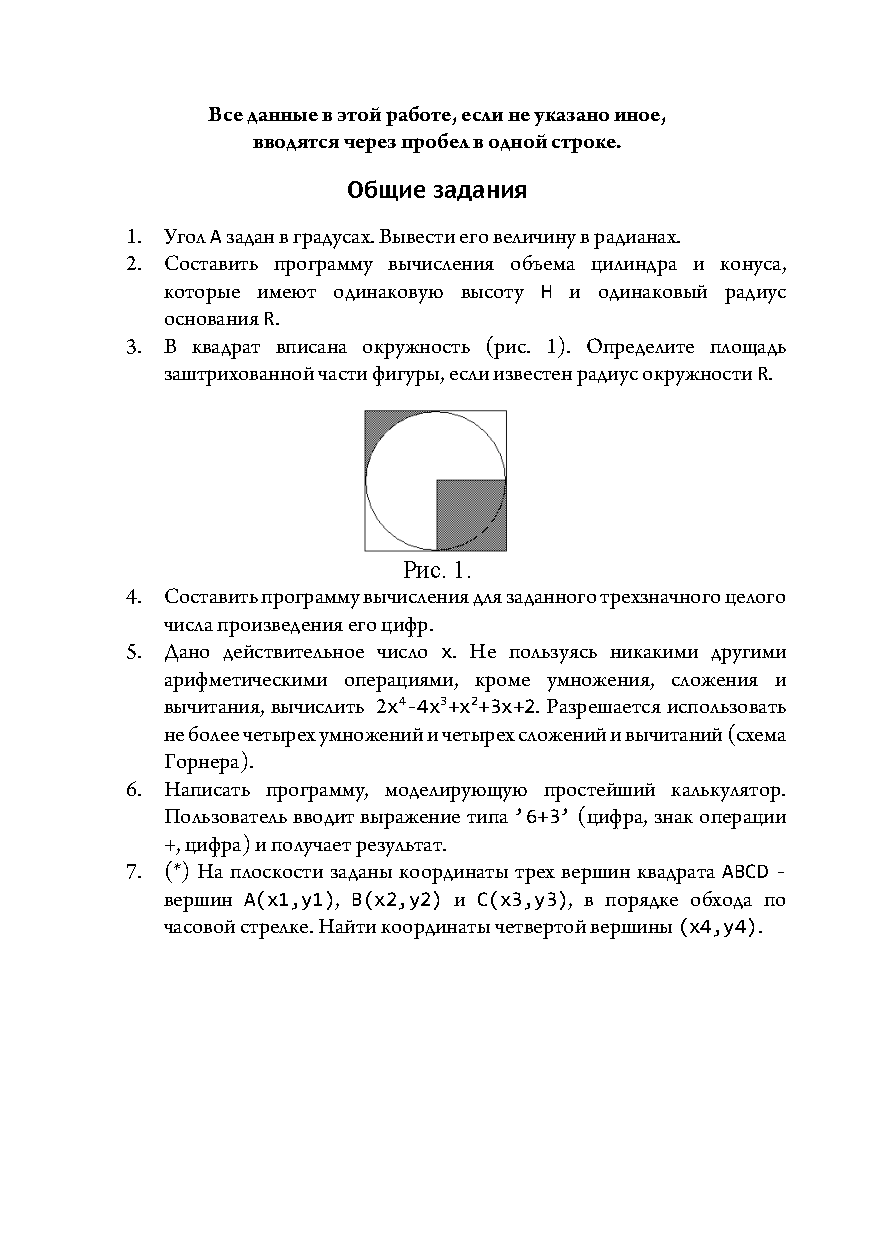
\includepdf[noautoscale,pages=-]{c01word}
\end{document}
